\chapter{معرفی الگوریتم
	\lr{Skein}
}
\section{
	مقدمه
}
دردنیای امروز، با افزایش لحظه‌ای اطلاعات در جهان، روز‌ به ‌روز رمزنگاری و رمزگذاری اطلاعات، اهمیت بیشتری پیدا می‌کند. برای مثال، برقراری امنیت سیستم‌ها و شبکه‌های رایانه‌ای، ذخیره‌ی اطلاعات مهم و حساس و ... همگی مثال‌هایی هستند که بدون رمزنگاری و رمزگذاری ممکن نخواهند بود. بی‌شک، بدون رمزگذاری و رمزنگاری، اینترنت به شکلی که امروز وجود دارد به هیچ عنوان وجود نمی‌داشت.
راه‌های بسیار متفاوتی برای رمزنگاری و رمزگذاری وجود دارد، یکی از مهم‌ترینِ آنها، استفاده از توابع رمزگذاری بر پایه‌ی
\textit{ 
	درهم‌سازی (
	\lr{Hashing}
	)
}
می باشد. درهم‌سازی به خودی خود پرکاربرد ترین داده‌ساختار استفاده شده در علوم رایانه‌ای است. برخی از توابع درهم‌سازی دارای ویژگی‌هایی هستند که آنهارا برای استفاده برای کاربرد‌هایی چون رمزنگاری بسیار مناسب می‌کند. مهم‌ترین و پرکاربردترین این توابع، توابعی از خانواده‌ی 
\textit{\lr{SHA}}
یا 
\textit{\lr{Secure Hashing Algorithms}}
می‌باشند، توابعی چون 
\lr{MD-5}
،
\lr{SHA-0}
،
\lr{SHA-1}
،
\lr{SHA-2}
و 
\lr{SHA-3}
که هر کدام خود شامل خانواده ای از توابع مخصوص کاربرد‌های خاص خود هستند.

توابع خانواده ی 
\lr{SHA}
توسط گروهی به نام 
\textit{\lr{NIST}}
که کوتاه شده‌ی عبارت
\textit{\lr{National Institute of Standards and Technology}}
است، برگزیده می‌شوند. برای انتخاب هریک از ورژن های توابع این خانواده، ابتدا توابعی پیشنهاد شده، پس از آن تعدادی از آنها به عنوان فینالیست توسط 
\lr{NIST}
اعلام شده و در نهایت از بین فینالیست‌ها، یک تابع به عنوان ورژن جدید از توابع 
\lr{SHA}
معرفی می‌شود.

تابع مورد بررسی در این مقاله یکی از توابع فینالیست برای انتخاب 
\lr{SHA-3}
می‌باشد که 
\lr{Skein}
نام دارد. 

\section{
	معرفی اجمالی الگوریتم
}
<<<<<<< HEAD
الگوریتم 
\textit{ \lr{Skein}}
  یکی از خانواده های توابع درهم سازی است که  بر‌اساس اندازه‌ی بلاک‌های داخلی سه نوع مختلف ۲۵۶ ، ۵۱۲  و ۱۰۲۴ بیتی دارد  .
  الگوریتم مورد بررسی در این مقاله مربوط به اندازه‌ی داخلی ۵۱۲ بیتی آن یعنی
  \lr{skein512}
  می‌باشد. در بین این سه نوع کلی از توابع
  \lr{skein}
  ،
 \lr{skein512}
 به عنوان تابع اصلی به کار می‌رود اما لازم به ذکر است که سرعت 
 \lr{skein1024}
دو برابر
 \lr{skein512}
 می‌باشد و 
  \lr{skein256}
 زمانی به کار می رود که نیازمند حجم کمی از رم  (حدود ۱۰۰ بایت) باشد .
 
  درحالت کلی توابع
    \lr{skein}
   توانایی درهم‌سازی ورودی به هر اندازه اندازه‌ای را دارد اما اندازه‌ی خروجی آن، معمولا یکی از حالت های ۲۵۶ یا ۵۱۲ یا ۱۰۲۴ بیتی است. 
  

\pagebreak
=======
\subsection{
	انواع
}
>>>>>>> origin/master
\section{
	روند اجرایی الگوریتم
}
ایده ی اصلی توابع \lr{Skein}  استفاده از
\textit{ \lr{Tweakable Block Ciphers}}
  یا بلاک های رمزگذاری قابل تنظیم است .
همه‌ی توابع 
\lr{skein}
از سه بخش کلی تشکیل شده اند:
\begin{itemize}
	\item 
	\lr{\textit{\textbf{Threefish}}} 
	یا بلاک های رمزنگاری قابل تنظیم
	\item
	\lr{
		\textit{
			\textbf{Unique Block Iteration (UBI)}
		}
	}

	\item
	\textbf{\lr{\textit{\textbf{Optional Argument System}}} } 
	
\end{itemize}
این سه بخش در کنار هم توابع درهم‌سازی
\lr{skein}
را تشکیل می‌دهند.
 در ادامه به تفصیل به عملکرد هریک از این بخش ها خواهیم‌ پرداخت.
 
\subsection{
	عملکرد
	\lr{Threefish}
}
در‌الگوریتم های 
 \lr{skein}
 بسته به نوع تابع درهم‌سازی از بلاک‌های رمزگذاری استفاده می‌شود که به صورت زنجیره‌ای به یکدیگر متصل شده‌اند، اندازه‌ی این بلاک‌ها بسته به نوع الگوریتم 
 ۲۵۶، ۵۱۲ یا ۱۰۲۴ بیت یا درواقع ۴، ۸ یا ۱۶ بسته‌ی ۶۴ بیتی از داده ها ‌می‌باشد. بلاک های رمزنگاری هرکدام از ترکیب دو تابع غیر خطی به نام های درهم‌سازی
 (
\textit{ \lr{Mix}}
 )
 و جابه‌جایی (
 \textit{ \lr{Permutation}}
)
تشکیل شده‌اند، هر بلاک رمزگذاری با بلاک‌های رمزگذاری دیگر سری شده و زنجیره ای از بلاک‌های رمزگذاری را تشکیل می‌دهند. علاوه براین بلاک‌ها، میان هر ۴ بلاک متوالی به مقادیر محاسبه شده تا آنجا مقادیر کلید هایی مربوط با آن دوره، افزوده می‌شود که به آنها 
\textit{\lr{Subkey}}
گفته‌میشود. در تصویر زیر شمایی کلی از فرایند توضیح داده‌شده قابل مشاهده است:
\begin{figure}[H]
	\centering
	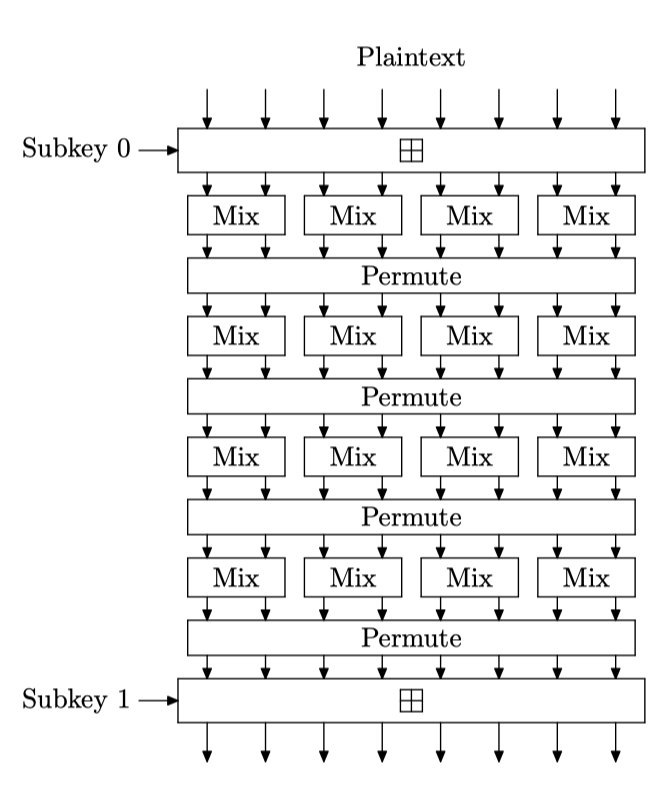
\includegraphics[width=7cm]{Images/Introduction/cipherblock_dataflow.png}	
	\caption{
		شمای کلی از کارکرد بلاک‌های رمزگذاری قابل تنظیم 
	}
\end{figure}
درادامه به توضیح هر‌یک از این توابع می‌پردازیم.
\pagebreak

\subsubsection{
تابع درهم‌سازی (
\lr{Mix}
)
}
این تابع غیر خطی دو بسته‌ی ۶۴ بیتی از داده‌ها ‌را به عنوان ورودی دریافت کرده و دو بسته‌ی ۶۴ بیتی دیگر که حاصلی از ترکیب دو بسته‌ی ورودی هستند را در خروجی تحویل می‌دهد.اگر بسته های ورودی به این تابع به ترتیب ارزش، 
$x_0$ 
و
$x_1$
باشند، بسته‌های خروجی این تابع از فورمول‌های زیر به دست می‌‌آیند:
$$y_0 = x_0 + x_1$$
$$y_1 = (x_0 + x_1) \oplus ( x_1 \lll R_{(d\ mod\  8),j})$$
و از لحاظ ساختار کلی، شمای حرکت داده در این تابع به شکل زیر خواهد بود:


\begin{figure}[H]
	\centering
	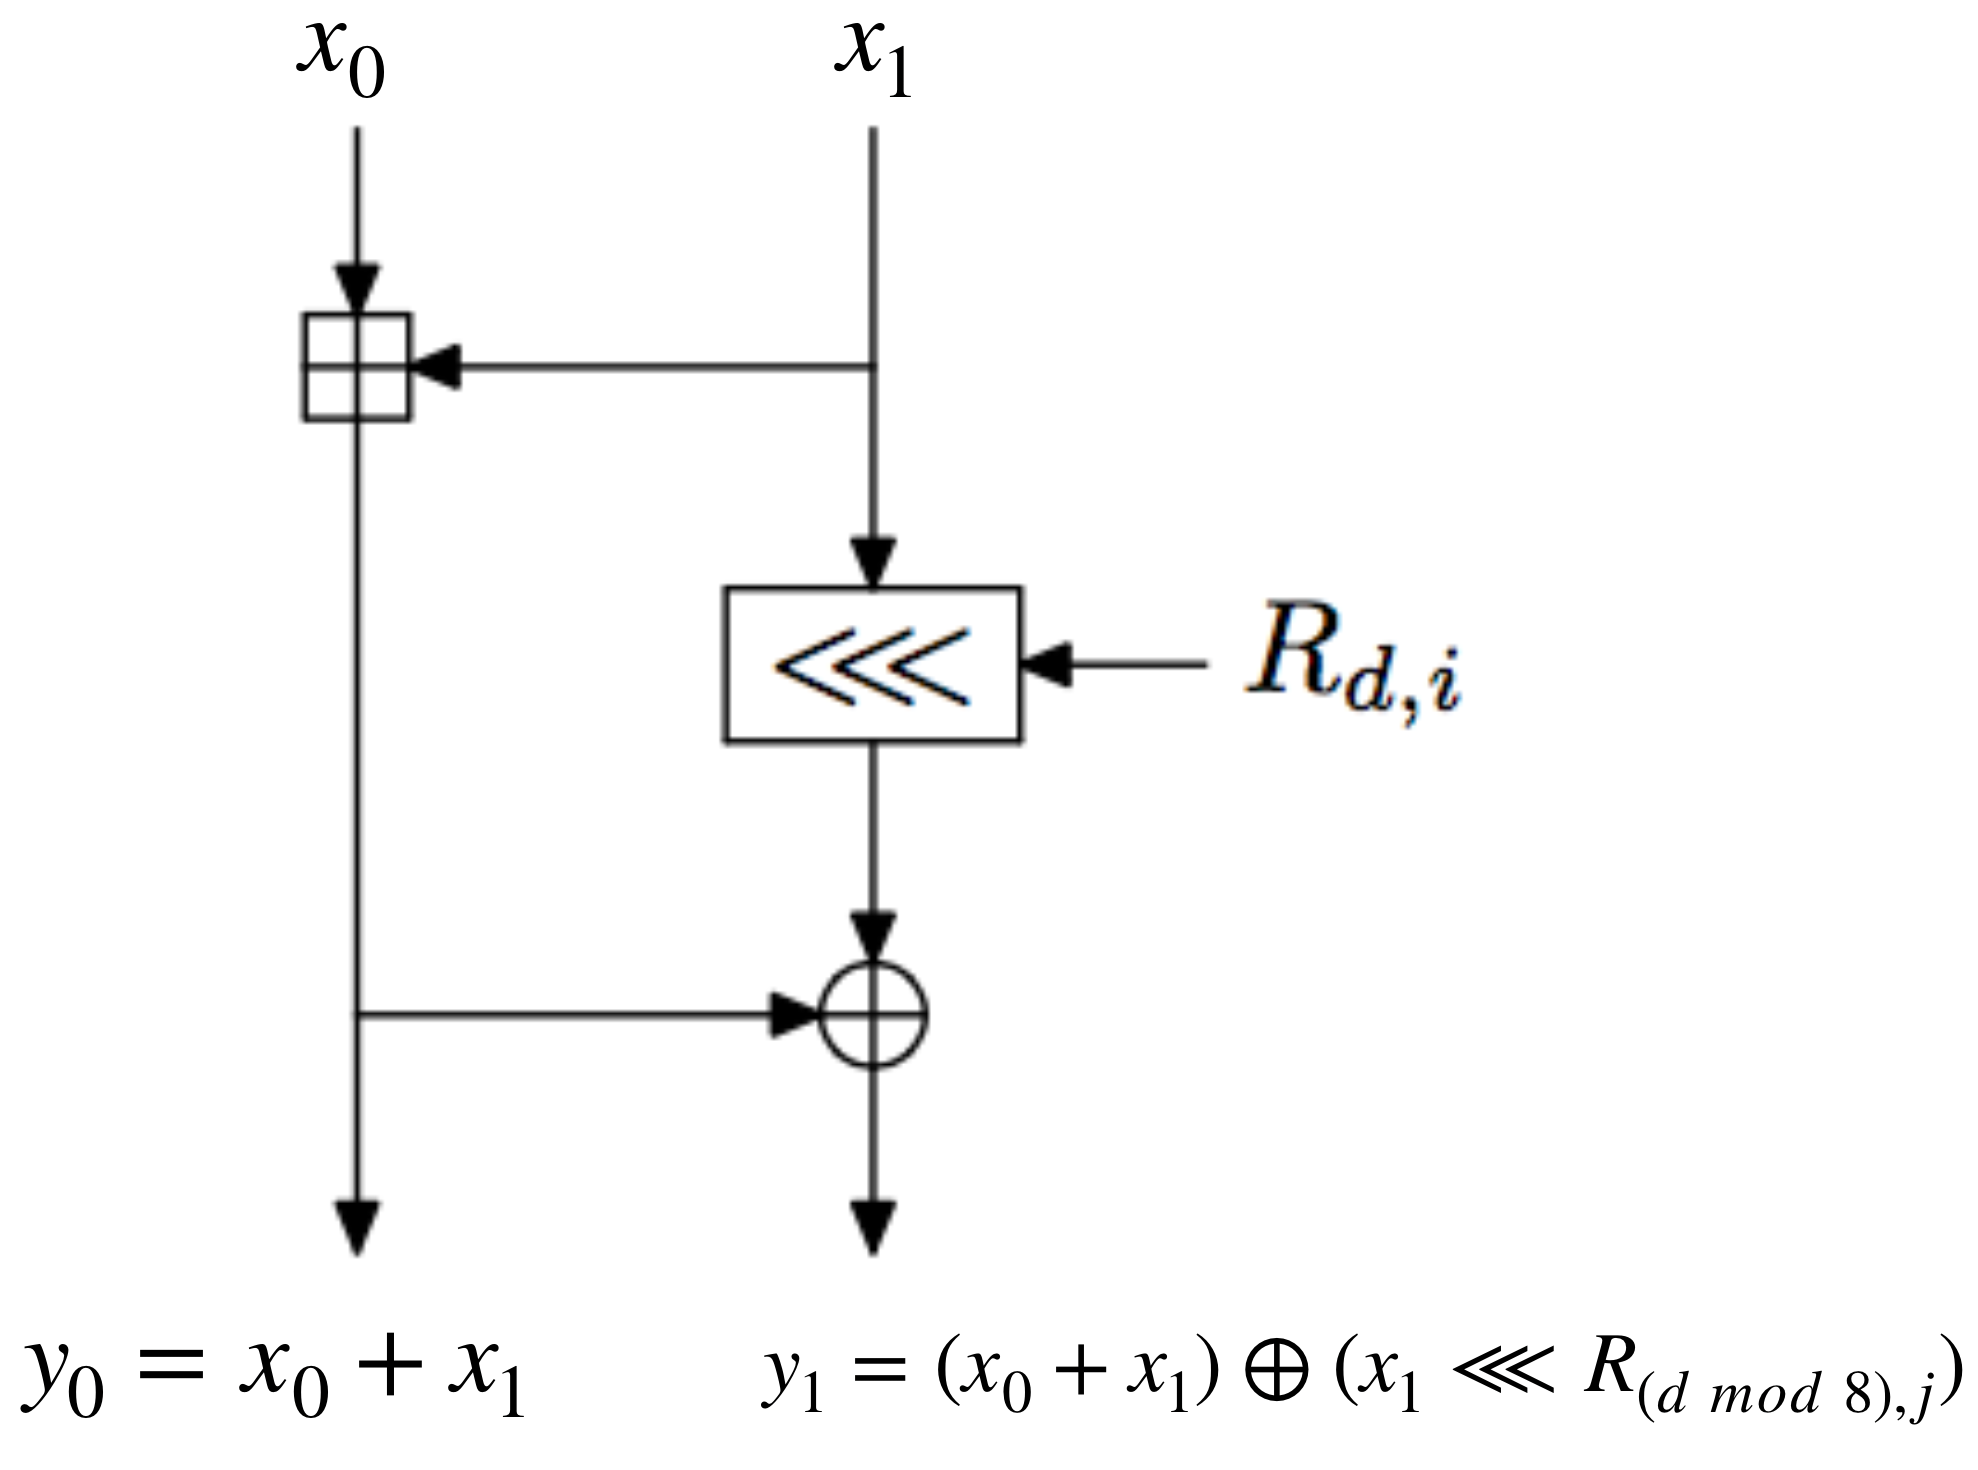
\includegraphics[width=7cm]{Images/Introduction/mix_function_dataflow.png}	
	\caption{
		شمای کلی از کارکرد تابع درهم‌سازی (\lr{Mix})
	}
\end{figure}


عدد
$d$
 شمارنده‌ی بلاک‌های رمزگذاری‌ می باشد که از صفر شروع شده است و عدد $j$ معرف شمارنده‌ی توابع درهم‌سازی (\lr{Mix}) داخل هر بلاک رمزگذاری است به صورتی که  عدد $j$  مربوط به تابعی که پرارزش‌ترین بسته‌های ورودی را دریافت می کند صفر و عدد $j$ مربوط به تابعی که کم‌ارزش‌ترین بسته‌ها را به عنوان ورودی دریافت می‌کند برابر 
$N_W/2 - 1$ 
‌باشد، که در آن 
$N_W$
تعداد بسته‌های موجود در بلاک‌های رمزگذاری است.


عدد 
$ R_{(d\ mod\  8),j}$
تعداد چرخش به چپ‌های لازم برای بسته‌ی ورودی دوم در تابع درهم‌سازی (\lr{Mix}) $j$ ام در بلاک رمزگذاری $d$ ام را مشخص می کند که مقدار آن  به ازای مقادیر مختلفی از 
$j$ و
$d$ و
$N_W$ 
در جدول زیر قابل مشاهده است:
  
  \begin{figure}[H]
  	\centering
  	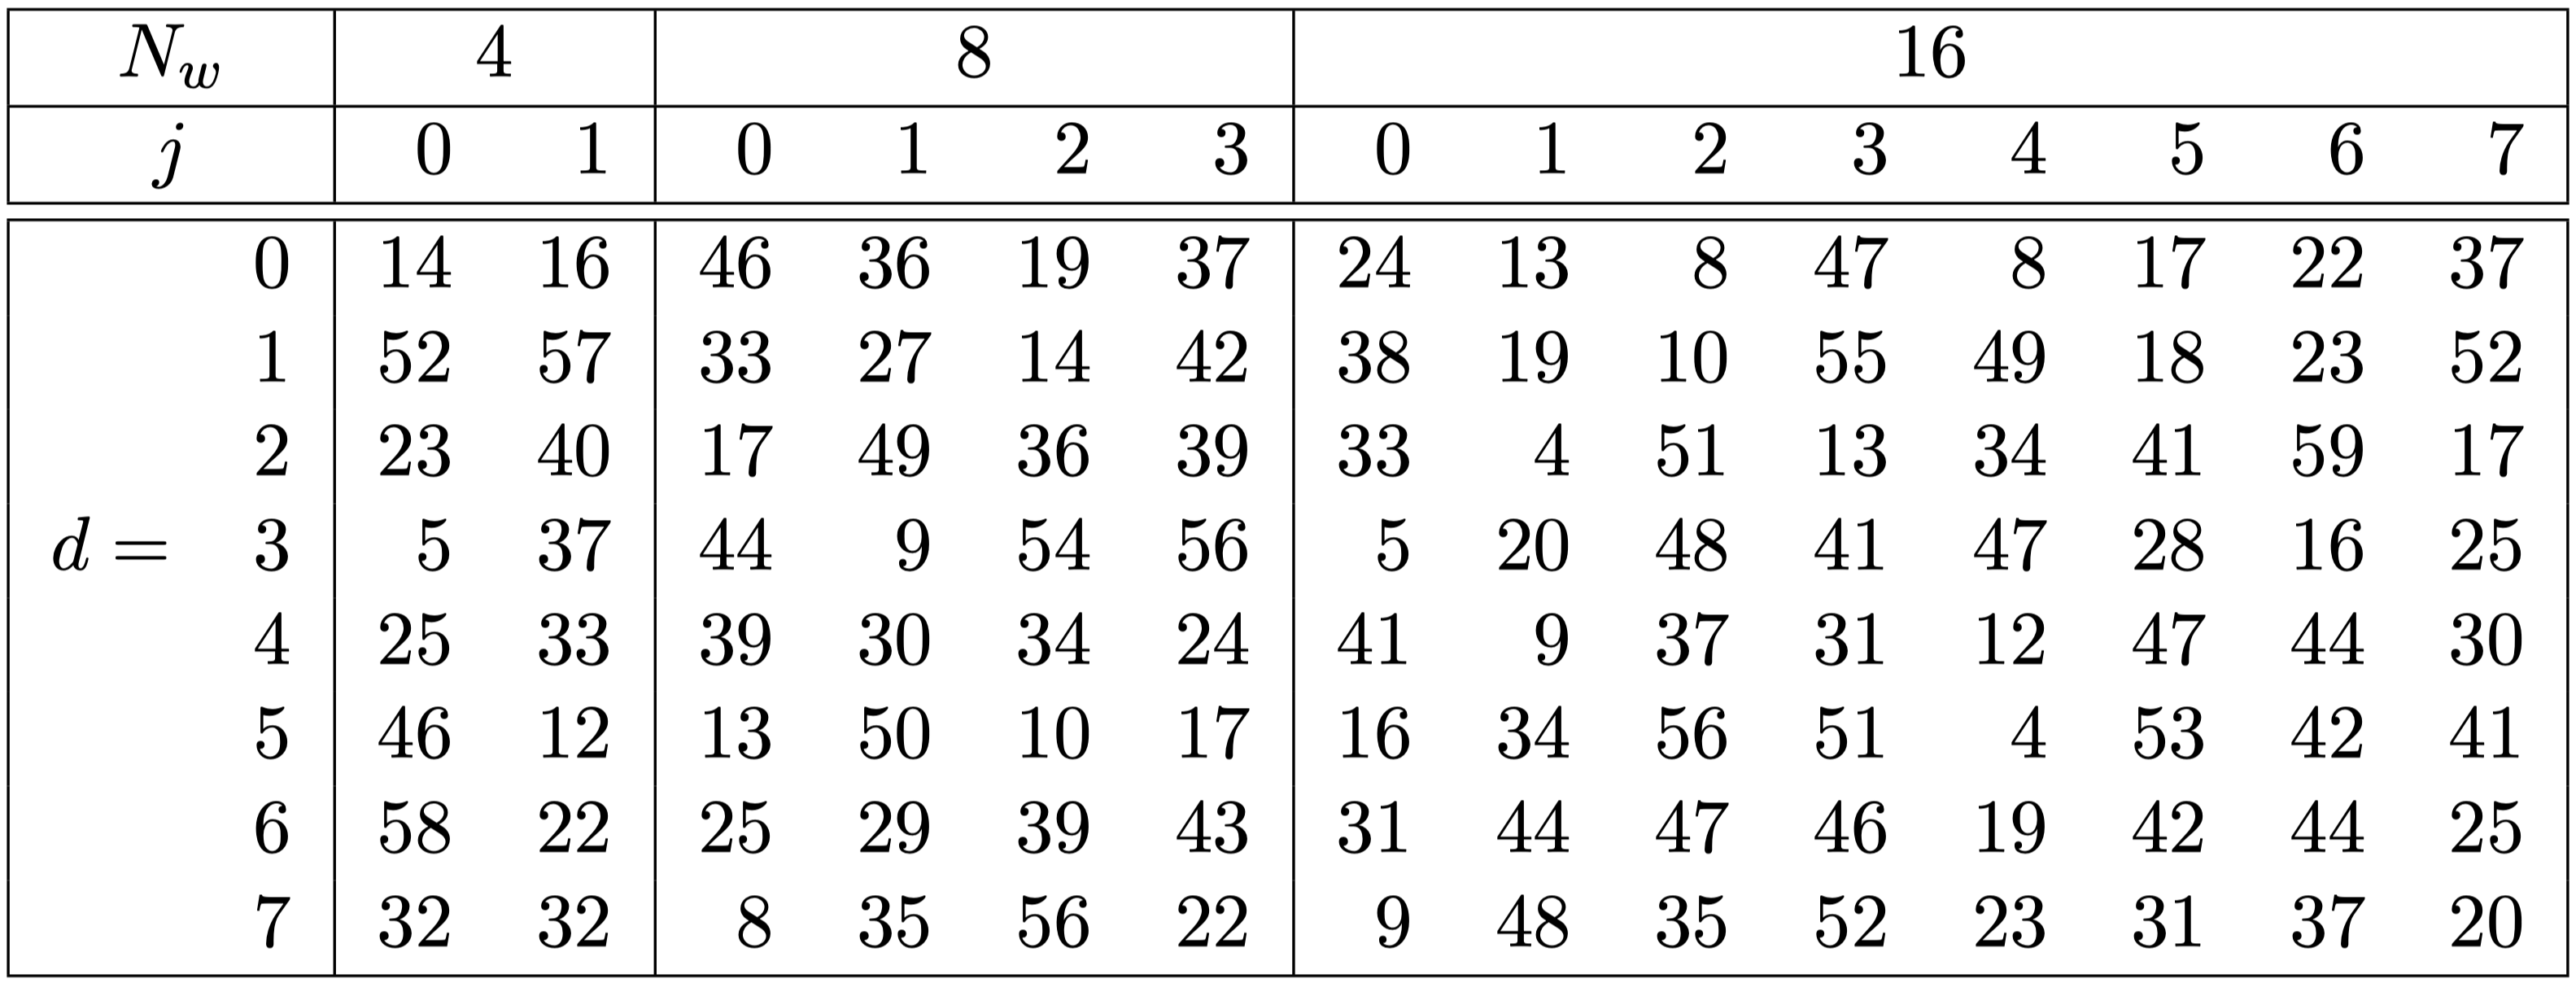
\includegraphics[width=15cm]{Images/Introduction/mix_function_rotate_values.png}	
  	\caption{جدول حاوی تعداد چرخش‌های صورت گرفته در تابع 
  	درهم‌سازی (\lr{Mix})
  }
  \end{figure}

\pagebreak
\subsubsection{
تابع جابه‌جایی (\lr{Permutation})
}
اگر فرض کنیم که خروجی های تابع درهم‌سازی (\lr{Mix}) $j$ در بلاک رمزگذاری $d$ ام، 
$f_{d,\ 2j}$
و
$f_{d,\ 2j+1}$
باشند، خروجی نهایی بلاک رمزگذاری یا در واقع ورودی بلاک رمزگذاری بعدی، برابر خروجی تابع غیر خطی جابه‌جایی (\lr{Permutation}) روی این مقادیر است که از رابطه ی زیر به دست می‌آید:
$$v_{d+1,\ i} = f_{d,\ \pi(i)}$$
که
$v$
معرف بسته‌ی اطلاعاتی ۶۴ بیتی و عدد
 $i$
  شماره‌ی آن بسته در بلاک رمزگذاری مربوط و  $\pi(i)$ یک تابع بوده که مقادیر آن در جدول زیر قابل مشاهده است:

 \begin{figure}[H]
	\centering
	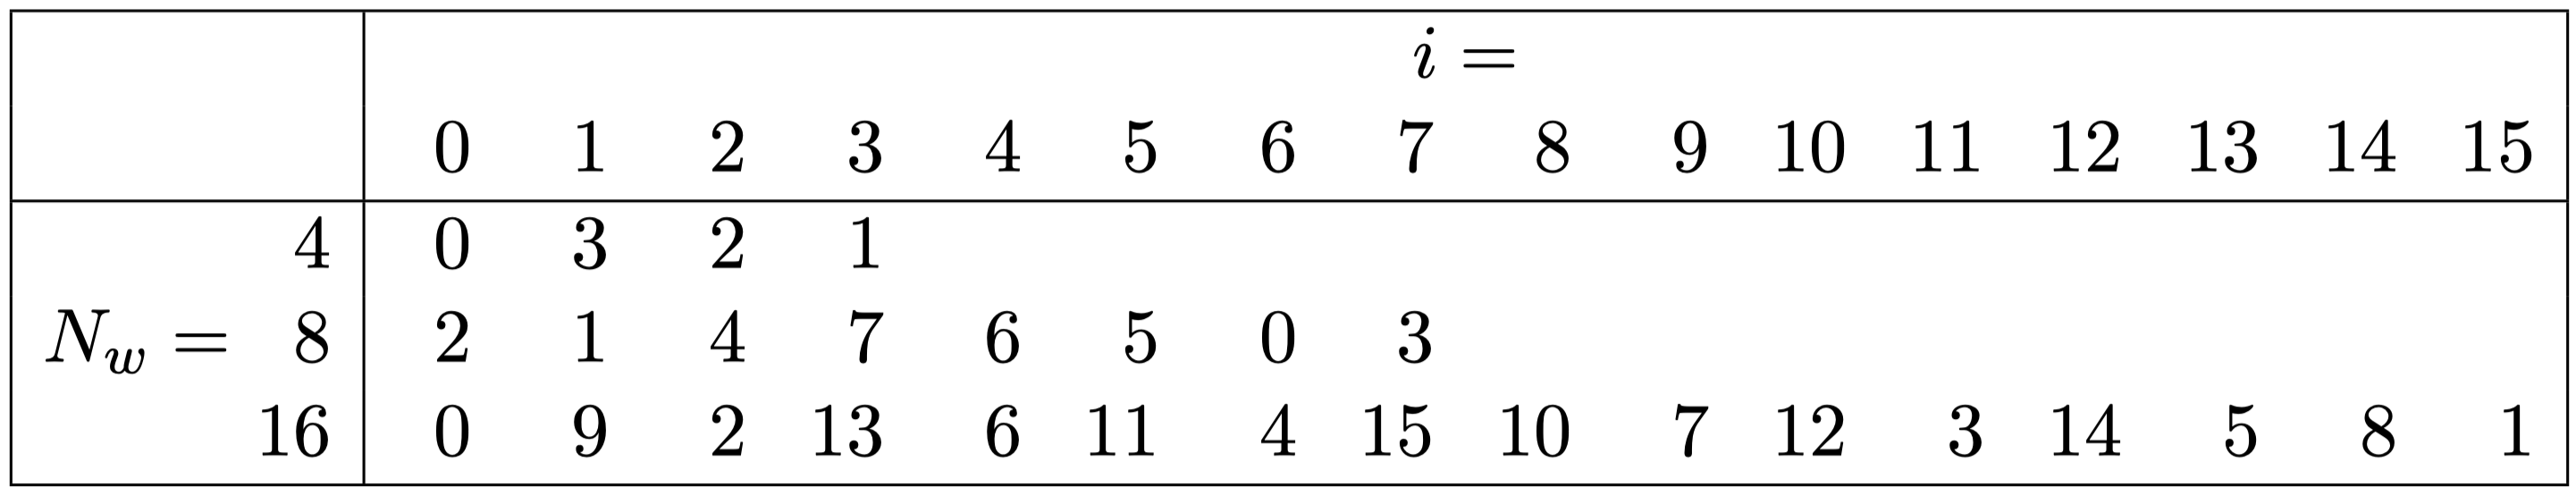
\includegraphics[width=15cm]{Images/Introduction/permutation_values.png}	
	\caption{جدول حاوی مقادیر
	$\pi(i)$
	برای محاسبه‌ی خروجی تابع جابه‌جایی (\lr{Permutation}) 
 }
\end{figure}
  
\subsubsection{
عملیات افزودن مقادیر کلید‌ها 
(\lr{Subkeys})
}

علاوه بر دادگان ورودی ( فرضا 
$p_0$ 
تا
$p_{N_W - 1}$
بسته های ۶۴ بیتی ورودی به کل بخش 
\lr{Threefish}
می‌باشند.
)
مقادیری به عنوان کلیدهای رمزگذاری (
$k_0$ 
تا
$k_{N_W - 1}$
که خود بسته‌های ۶۴ بیتی اند
)
و
دو بسته‌ی ۶۴ بیتی 
$t_0$ 
و
$t_1$
به عنوان تنظیم (
\lr{Tweak}
) 
نیز به ‌بخش 
\lr{Threefish}
در این الگوریتم داده می‌شوند. این مقادیر اضافه پیش از هر ۴ بلاک رمزگذاری با مقادیر خروجی از بلاک رمزگذاری قبل ترکیب می‌شوند. درواقع ورودی بلاک رمزگذاری $d$ ام از رابطه ی زیر به دست می‌آید:
\begin{figure}[H]
	\centering
	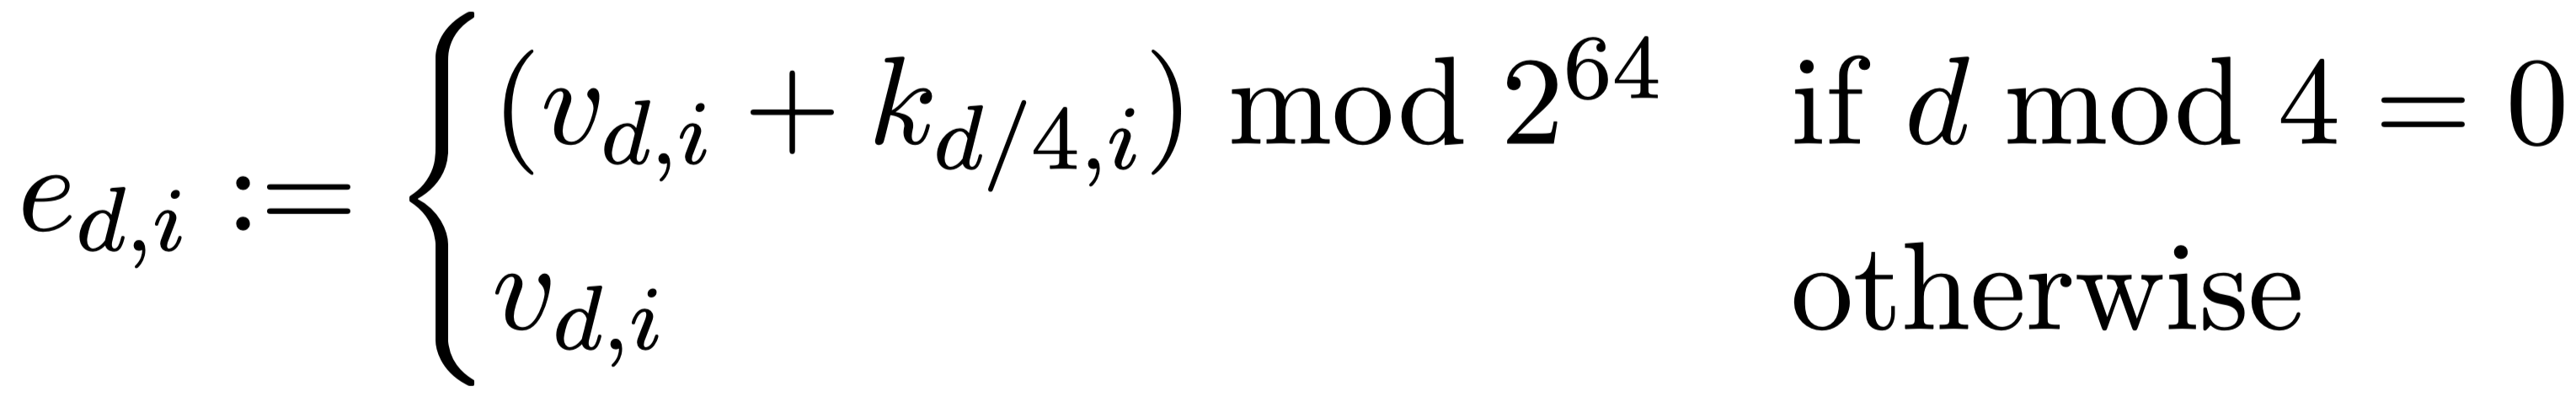
\includegraphics[width=7cm]{Images/Introduction/subkey_equation_1.png}	
	
\end{figure}
که $i$ در شماره‌ی بسته‌ی ۶۴ بیتی اطلاعات است و $v_{0,i}$ ها همان بسته های ۶۴ بیتی ورودی به کل بخش 
\lr{Threefish}
یعنی 
$p_0$ 
تا
$p_{N_W - 1}$
می‌باشند  و مقدار $k$ ها نیز با‌توجه به روابط زیر قابل مقایسه است:
	\begin{latin}
		\begin{center}
			\begin{tabular}{l l}
				$k_{s, i} = k_{(s+i) \mod\ N_W+1} $ \hspace{15mm} & $  i = 0,\ 1,\ 2,\ ... ,\ N_W-4 $ \\
				$k_{s, 5} = k_{(s+5) \mod\ N_W+1} + t_{s \mod 3}$ & \\
				$k_{s, 6} = k_{(s+6) \mod\ N_W+1} + t_{(s+1) \mod 3}$ & \\
				$k_{s, 7} = k_{(s+7) \mod\ N_W+1} + s $ & \\
				
			\end{tabular}
		\end{center}
	\end{latin}

<<<<<<< HEAD
که در این روابط مقادیر $k_{N_W}$ و
$t_2$
از قرار زیر اند:
$$
k_{N_W} = C_{240} \oplus k_0 \oplus k_1 \oplus ... \oplus k_{N_W - 1}
$$

$$
t_2 = t_1 \oplus t_0
$$
که $ C_{240} $ عددی ثابت و برابر \lr{0x1BD11BDAA9FC1A22} است و به آن جهت در فرمول وجود دارد که از ۰ نبودن تمامی بیت‌ها اطمینان حاصل شود.

\subsection{
	\lr{Unique Block Iteration (UBI)}
}

\subsection{
	\lr{Optional Argument System}
}
=======
>>>>>>> origin/master
